% !TeX program = xelatex
\documentclass[12pt,a4paper]{article}
% !TeX root = ../main.tex
\usepackage{fontspec}
% Text width: 81 mm + 6 mm + 81 mm. Top margin is a project setting.
\usepackage[a4paper,left=21mm,right=21mm,top=25mm,bottom=29mm]{geometry}
\usepackage{amsmath}
\usepackage{unicode-math}
\usepackage{array}
\usepackage{tabularx}
\usepackage{graphicx}
\usepackage{pdflscape}
\usepackage{tikz}
\usetikzlibrary{arrows.meta}
\usepackage{float}
\usepackage{placeins}
\usepackage{titlesec}
\usepackage{caption}
\usepackage{indentfirst}
\usepackage{cite}
\usepackage{balance}
\usepackage[unicode,hidelinks]{hyperref}
\urlstyle{same}
\setmainfont{Angsana New}[Script=Thai]
\setsansfont{Angsana New}[Script=Thai]
% Times-style mathematics complements the Latin letters in Angsana New.
\setmathfont{texgyretermes-math.otf}
\XeTeXlinebreaklocale "th"
% Preserve original Thai Unicode when copying/searching shaped glyphs in the PDF.
\XeTeXgenerateactualtext=1
\XeTeXlinebreakskip=0pt plus 1pt
\graphicspath{{images/}}
\setlength{\columnsep}{6mm}
\setlength{\parindent}{12.7mm}
\setlength{\parskip}{0pt}
\setlength{\textfloatsep}{16bp}
\setlength{\dbltextfloatsep}{16bp}
\setlength{\dblfloatsep}{16bp}
\setlength{\intextsep}{16bp}
\setlength{\emergencystretch}{3em}
% Wide research diagrams and tables float at page tops in two-column mode.
\renewcommand{\dbltopfraction}{0.85}
\renewcommand{\topfraction}{0.85}
\renewcommand{\textfraction}{0.1}
\renewcommand{\floatpagefraction}{0.75}
\renewcommand{\dblfloatpagefraction}{0.75}
% Number the report for reading/review; conference camera-ready rules may differ.
\setlength{\footskip}{12mm}
\pagestyle{plain}
\renewcommand{\figurename}{ภาพที่}
\renewcommand{\tablename}{ตารางที่}
\renewcommand{\refname}{เอกสารอ้างอิง}
\renewcommand{\appendixname}{ภาคผนวก}
\makeatletter
\renewcommand{\normalsize}{\@setfontsize\normalsize{12bp}{16bp}}
\makeatother
\AtBeginDocument{\normalsize}
% Keep both inline and display mathematics close to the body text's visual size.
\DeclareMathSizes{12bp}{10bp}{7bp}{5bp}
\titleformat{\section}{\fontsize{14bp}{16bp}\selectfont\bfseries\raggedright}{\thesection.}{0.5em}{}
\titleformat{\subsection}{\fontsize{14bp}{16bp}\selectfont\bfseries\raggedright}{\thesubsection}{0.5em}{}
\titleformat{\subsubsection}{\fontsize{14bp}{16bp}\selectfont\bfseries\raggedright}{\thesubsubsection}{0.5em}{}
\titlespacing{\section}{0pt}{16bp}{0pt}
\titlespacing{\subsection}{0pt}{16bp}{0pt}
\titlespacing{\subsubsection}{0pt}{16bp}{0pt}
\DeclareCaptionFont{articlebody}{\fontsize{12bp}{16bp}\selectfont}
\captionsetup{font=articlebody,labelsep=space,skip=0pt}
\captionsetup[table]{position=top,justification=raggedright,singlelinecheck=false}
\renewcommand{\maketitle}{%
  \begin{center}
    {\fontsize{16bp}{20bp}\selectfont\bfseries
      \ArticleTitleTH\par
      \ArticleTitleEN\par}
    \vspace{16bp}
    {\fontsize{12bp}{16bp}\selectfont\bfseries
      \ArticleAuthor\par
      \ArticleAffiliation\par}
    \ArticleAddress\par % contact information awaits author confirmation

  \end{center}
  \vspace{16bp}
}

% ข้อมูลผู้เขียนจาก PreProject .docx; ยังไม่ระบุข้อมูลติดต่อที่ไม่ยืนยัน
\newcommand{\ArticleTitleTH}{ระบบลานิสิตสำหรับคณะวิศวกรรมศาสตร์ กำแพงแสน}
\newcommand{\ArticleTitleEN}{Student Leave Management System for the Faculty of Engineering at Kamphaeng Saen}
\newcommand{\ArticleAuthor}{จิรภัทร แซ่ลี้ และ กานตภัท อาจหาญ}
\newcommand{\ArticleAffiliation}{ภาควิชาวิศวกรรมคอมพิวเตอร์ คณะวิศวกรรมศาสตร์ กำแพงแสน มหาวิทยาลัยเกษตรศาสตร์ วิทยาเขตกำแพงแสน}
\newcommand{\ArticleAddress}{1 หมู่ 6 ต.กำแพงแสน อ.กำแพงแสน จ.นครปฐม 73140}
\newcommand{\ArticleAdvisor}{อ.ธีรวัฒน์ หวายฤทธิ์ (อาจารย์ที่ปรึกษาหลัก)}
\newcommand{\ArticleCoAdvisor}{ผศ.ดร.วรัญญา อรรถเสนา (อาจารย์ที่ปรึกษารอง)}

\begin{document}
\twocolumn[\maketitle]
\section*{บทคัดย่อ}
บทความนี้นำเสนอการออกแบบและพัฒนาระบบลานิสิตสำหรับคณะวิศวกรรมศาสตร์ กำแพงแสน มหาวิทยาลัยเกษตรศาสตร์ เพื่อรวมการยื่นคำขอ การแนบหลักฐาน การพิจารณาตามลำดับ และการติดตามสถานะไว้ในเว็บแอปพลิเคชันเดียว ระบบใช้ Next.js สำหรับส่วนติดต่อผู้ใช้ NestJS สำหรับบริการฝั่งเซิร์ฟเวอร์ และ Prisma เชื่อมต่อฐานข้อมูล การเข้าถึงคำขอและรายงานจำกัดตามตัวตนผู้ใช้ บทบาท และความสัมพันธ์กับนิสิต ระบบข้อมูลสนับสนุน จัดการข้อมูลรายวิชา ผู้สอน และที่ปรึกษา ส่วนคลังข้อมูลรายงานแยกจากข้อมูลธุรกรรมเพื่อรองรับการสรุปจำนวนใบลา วันลา และรายวิชาที่ได้รับผลกระทบ ผลการตรวจซอร์สโค้ดพบองค์ประกอบรองรับกระบวนการหลักและการควบคุมสิทธิ์ดังกล่าว อย่างไรก็ตาม ยังต้องประเมินการใช้งานกับผู้ใช้จริงและทดสอบประสิทธิภาพก่อนสรุปผลเชิงปริมาณ
\par\noindent\textbf{คำสำคัญ:} ระบบลานิสิต, เว็บแอปพลิเคชัน, การอนุมัติ
\section*{Abstract}
This article presents the design and implementation of a student leave management system for the Faculty of Engineering at Kamphaeng Saen, Kasetsart University. The system integrates request submission, evidence attachments, sequential approval, and status tracking in a web application. Next.js provides the user interface, while NestJS and Prisma support server services and database access. Request and report access is scoped by user identity, role, and relationships with students. A separate Student Leave Reference Data Management System manages subject, lecturer, and advisor reference data. The reporting warehouse is separated from operational transactions to summarize requests, leave days, and affected subjects. Source code inspection identifies support for these core workflows and access controls. User evaluation and performance testing remain necessary before quantitative benefits can be established.
\par\noindent\textbf{Keywords:} student leave, web application, approval workflow

\section{บทนำ}
การลาหยุดเรียนของนิสิตเกี่ยวข้องกับข้อมูลส่วนบุคคล ช่วงเวลาที่ลา รายวิชาที่ขาดเรียน และการพิจารณาจากผู้รับผิดชอบหลายฝ่าย ข้อเสนอโครงงานระบบลานิสิตระบุว่าการใช้เอกสารหรือข้อมูลที่แยกกันอาจทำให้ติดตามสถานะได้ยาก เกิดความซ้ำซ้อน และค้นหาประวัติย้อนหลังไม่สะดวก \cite{proposal} จึงมีความจำเป็นต้องจัดเก็บคำขอและประวัติการพิจารณาในระบบเดียว
โครงงานนี้มีวัตถุประสงค์เพื่อพัฒนาเว็บแอปพลิเคชันสำหรับยื่นและติดตามคำขอลา สนับสนุนการพิจารณาตามลำดับหน้าที่ และจัดทำรายงานภายใต้สิทธิ์ของผู้ใช้งาน ขอบเขตครอบคลุมนิสิต อาจารย์ที่ปรึกษา ผู้อนุมัติระดับภาควิชาและคณะ อาจารย์ผู้สอน และเจ้าหน้าที่ โดยข้อมูลระบุตัวตนและข้อมูลทางการศึกษาบางส่วนอาศัยบริการภายนอกของหน่วยงาน
บทความนี้อธิบายระบบจากข้อเสนอโครงงานร่วมกับซอร์สโค้ดที่ตรวจครั้งแรกเมื่อวันที่ 15 ตุลาคม 2569 และตรวจทานความสอดคล้องอีกครั้งเมื่อวันที่ 21 ตุลาคม 2569 \cite{repo} ผลที่รายงานจึงเป็นผลการตรวจองค์ประกอบและตรรกะของระบบ มิใช่ผลทดลองกับประชากรนิสิตหรือหลักฐานว่าระบบลดเวลาและต้นทุนได้แล้ว

\input{sections/02-related-work}
\section{การออกแบบและพัฒนาระบบ}
\subsection{สถาปัตยกรรมของระบบ}
\begin{figure}[H]
\centering
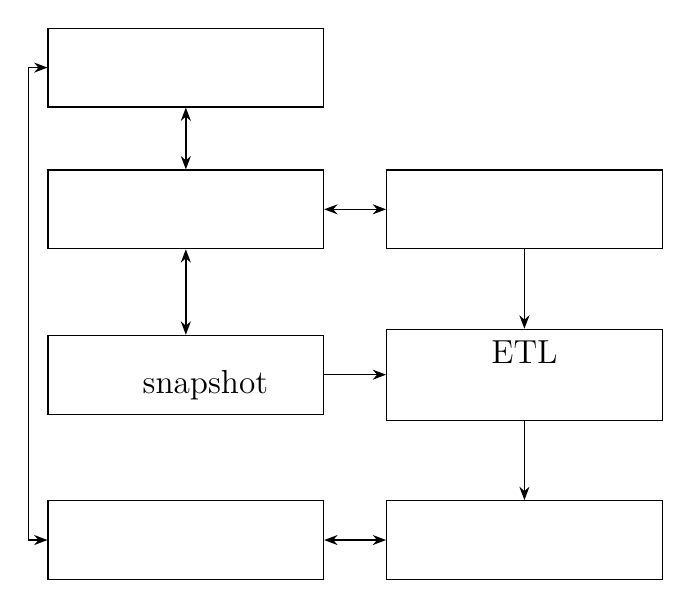
\begin{tikzpicture}[
  x=1mm,y=1mm,
  box/.style={draw,rectangle,align=center,text width=32mm,minimum height=10mm,inner sep=1.5mm,font=\fontsize{12bp}{16bp}\selectfont},
  flow/.style={-{Stealth[length=1.7mm]},line width=0.5pt},
  exchange/.style={{Stealth[length=1.7mm]}-{Stealth[length=1.7mm]},line width=0.5pt}
]
\node[box] (web) at (0,0) {ผู้ใช้ผ่านเว็บระบบใบลา};
\node[box] (api) at (0,-18) {บริการระบบใบลา};
\node[box] (support) at (43,-18) {ระบบข้อมูลสนับสนุน\\วิชา ผู้สอน ที่ปรึกษา};
\node[box] (db) at (0,-39) {ฐานข้อมูลใบลา\\และ snapshot};
\node[box] (etl) at (43,-39) {ETL\\ตรวจและแปลงข้อมูล};
\node[box] (report) at (0,-60) {บริการรายงาน\\ตรวจสิทธิ์ก่อนส่งผล};
\node[box] (dw) at (43,-60) {คลังข้อมูลรายงาน};
\draw[exchange] (web) -- (api);
\draw[exchange] (api) -- (support);
\draw[exchange] (api) -- (db);
\draw[flow] (db) -- (etl);
\draw[flow] (support) -- (etl);
\draw[flow] (etl) -- (dw);
\draw[exchange] (report) -- (dw);
\draw[exchange] (report.west) -- (-20,-60) -- (-20,0) -- (web.west);
\end{tikzpicture}
\caption{องค์ประกอบและการเชื่อมต่อข้อมูลของระบบ}\label{fig:architecture}
\end{figure}
ส่วนติดต่อผู้ใช้พัฒนาด้วย Next.js และ React ส่วนบริการประมวลผลใช้ NestJS และเข้าถึงฐานข้อมูลผ่าน Prisma ตามแฟ้มกำหนดแพ็กเกจและสคีมาในโครงการ ระบบเชื่อมบริการยืนยันตัวตน บุคลากร และข้อมูลประกอบใบลาจากภายนอก โดยการตั้งค่าปลายทางและข้อมูลลับอยู่ฝั่งเซิร์ฟเวอร์ แผนภาพสรุปองค์ประกอบหลักอยู่ในภาพที่~\ref{fig:architecture} ลูกศรสองทางหมายถึงการเรียกบริการและรับผล ส่วนลูกศรทางเดียวหมายถึงการส่งข้อมูลเข้าสู่กระบวนการรายงาน โดยบริการรายงานตรวจขอบเขตผู้ใช้กับต้นทางก่อนส่งผลให้หน้าเว็บ

\subsubsection{เทคโนโลยีส่วนติดต่อผู้ใช้}
เว็บระบบใบลาและระบบข้อมูลสนับสนุนใช้ Next.js และ React สำหรับสร้างหน้าเว็บร่วมกับ TypeScript เพื่อจัดการโครงสร้างข้อมูล ส่วนติดต่อแบ่งเป็นหน้าสำหรับนิสิต อาจารย์ และผู้ดูแลระบบตามหน้าที่ของแต่ละกลุ่ม \cite{repo}
ส่วนติดต่อใช้ Tailwind CSS 4 ร่วมกับคอมโพเนนต์แนวทาง shadcn/ui และ Radix UI เพื่อประกอบแบบฟอร์ม ตาราง และกล่องโต้ตอบ การแยกคอมโพเนนต์ช่วยให้หน้าสำหรับนิสิต อาจารย์ และผู้ดูแลระบบใช้รูปแบบร่วมกันได้ ขณะที่ตรรกะเฉพาะบทบาทยังแยกในหน้าหรือบริการที่เกี่ยวข้อง
แบบฟอร์มยื่นใบลาใช้ React Hook Form จัดการค่าช่องกรอกและสถานะฟอร์ม ร่วมกับ Zod และ resolver สำหรับตรวจรูปแบบข้อมูลก่อนส่ง การตรวจฝั่งหน้าเว็บช่วยให้แจ้งข้อผิดพลาดใกล้ช่องกรอก แต่ไม่แทนการตรวจเงื่อนไขและสิทธิ์ฝั่งเซิร์ฟเวอร์ Axios ใช้รับส่งข้อมูลกับบริการ ส่วน Recharts ใช้สร้างกราฟรายงาน และส่วนเอกสารใช้ html-to-image ร่วมกับ jsPDF ในขั้นตอนส่งออกเอกสาร
\subsubsection{เทคโนโลยีบริการและการจัดเก็บ}
บริการทั้งสองโครงการใช้ NestJS บน Node.js โดยแยกส่วนรับคำขอ กฎการทำงาน และความสามารถแต่ละด้าน เช่น ใบลา ข้อมูลสนับสนุน และรายงาน โครงสร้างนี้ทำให้ตรรกะการเปลี่ยนสถานะไม่จำเป็นต้องอยู่ในหน้าเว็บ และใช้ซ้ำได้จากผู้เรียกที่ได้รับสิทธิ์
Prisma เชื่อมต่อฐานข้อมูล MySQL เพื่อจัดเก็บและค้นหาข้อมูลที่สัมพันธ์กัน ส่วนการเขียนคำขอกับขั้นอนุมัติใช้ธุรกรรมเพื่อรักษาความสอดคล้อง Multer รองรับการรับแฟ้มผ่านบริการฝั่งเซิร์ฟเวอร์ โดยการตรวจเจ้าของและสถานะคำขอเป็นตรรกะอีกส่วนหนึ่งของระบบใบลา
ตารางที่~\ref{tab:tech-stack} สรุปเทคโนโลยีตามหน้าที่ เพื่อแยกเฟรมเวิร์กส่วนติดต่อ เครื่องมือจัดเก็บ และเครื่องมือวิเคราะห์ออกจากกัน รายการแพ็กเกจที่มีอยู่เพียงอย่างเดียวไม่ใช่หลักฐานว่าทุกความสามารถถูกเปิดใช้ในการติดตั้งจริง
\begin{table}[H]
\caption{เทคโนโลยีหลักและหน้าที่ในระบบ}\label{tab:tech-stack}
\centering
\begin{tabularx}{\columnwidth}{|p{30mm}|X|}
\hline
เทคโนโลยี & หน้าที่ \\ \hline
Next.js / React & หน้าเว็บและคอมโพเนนต์ผู้ใช้ \\ \hline
Tailwind / shadcn/ui & รูปแบบและองค์ประกอบหน้าจอ \\ \hline
React Hook Form / Zod & จัดการและตรวจข้อมูลแบบฟอร์ม \\ \hline
NestJS / TypeScript & บริการและกฎการทำงาน \\ \hline
Prisma / MySQL & เชื่อมข้อมูลและจัดเก็บธุรกรรม \\ \hline
Recharts & กราฟสถิติการลา \\ \hline
xlsx & อ่านข้อมูล Excel ในระบบสนับสนุน \\ \hline
Node.js / SQL & ประมวลผล ETL และคลังข้อมูล \\ \hline
\end{tabularx}
\end{table}
\subsubsection{เทคโนโลยีข้อมูลสนับสนุนและคลังข้อมูล}
บริการนำเข้าของระบบข้อมูลสนับสนุนใช้ไลบรารี xlsx อ่าน workbook และแปลงแถวเป็นข้อมูลวิชา ตอนเรียน ผู้สอน หรือที่ปรึกษา ก่อนเขียนด้วย Prisma การจัดการรูปแบบ Excel จึงเป็นหน้าที่ของบริการนำเข้า ส่วนกฎรายการซ้ำและความสัมพันธ์อาศัยทั้งตรรกะโปรแกรมและคีย์ของฐานข้อมูล
คลังข้อมูลใช้ Node.js จัดเตรียมข้อมูลสำหรับรายงาน โดยแยกการรวบรวม ตรวจสอบ และนำเข้าข้อมูลออกจากงานยื่นใบลา ช่วยให้กำหนดวิธีรวมยอดและปรับปรุงรายงานได้อย่างเป็นระบบ อีกทั้งลดการคำนวณรายงานซ้ำจากข้อมูลที่กำลังใช้พิจารณาคำขอ
\subsubsection{เครื่องมือพัฒนาและการติดตั้ง}
โครงการจัดเป็น pnpm monorepo แยก apps/web และ apps/api และมี lockfile ควบคุมการติดตั้ง dependency ระบบใบลาระบุ Node.js 22 และ pnpm 10.0.0 ในคู่มือและ Dockerfile โดยมี image สำหรับเว็บและบริการแยกกัน การแยกส่วนนี้ทำให้กำหนดตัวแปรแวดล้อมและพื้นที่เก็บแฟ้มของแต่ละบริการได้ตามหน้าที่
ESLint และ TypeScript ใช้ตรวจซอร์สโค้ด ส่วนชุดทดสอบสิทธิ์และ ETL ของระบบใบลาใช้ตัวทดสอบของ Node.js สำหรับระบบข้อมูลสนับสนุนมีการกำหนด Jest และ Supertest ในโครงการ การกล่าวถึงเครื่องมือเหล่านี้เป็นคำอธิบายสิ่งที่มีในโค้ด ไม่ใช่รายงานว่ารันผ่านทุกชุดในการจัดทำบทความครั้งนี้
\subsection{ระบบข้อมูลสนับสนุน}
ระบบข้อมูลสนับสนุนการลานิสิต คณะวิศวกรรมศาสตร์ กำแพงแสน (Student Leave Reference Data Management System) จัดการข้อมูลรายวิชา ตอนเรียน ผู้สอน และความสัมพันธ์ระหว่างที่ปรึกษากับนิสิตแยกจากข้อมูลคำขอลา ระบบใบลาเรียกใช้ข้อมูลเหล่านี้เพื่อประกอบแบบฟอร์ม เลือกวิชาและผู้สอน ตลอดจนตรวจขอบเขตนิสิตในความดูแล \cite{components}
ข้อมูลรายวิชารองรับหลายตอนเรียนและผู้สอนร่วม มีการเก็บตารางเรียน วันเรียน และช่วงเวลาเพื่อระบุว่าการลาส่งผลต่อการเรียนวิชาใดบ้าง ส่วนข้อมูลที่ปรึกษาช่วยกำหนดผู้พิจารณาขั้นแรกและขอบเขตรายงาน ความสัมพันธ์เหล่านี้จึงใช้ทั้งในการยื่นคำขอและการเข้าถึงข้อมูลตามหน้าที่
ผู้ดูแลข้อมูลสามารถนำเข้ารายวิชาและข้อมูลที่ปรึกษาจาก Excel โดยเลือกเพิ่มรายการใหม่หรือแทนที่ชุดเดิม ระบบตรวจรายการซ้ำและความสัมพันธ์ก่อนบันทึก การแยกงานนำเข้าออกจากการยื่นใบลาช่วยให้ปรับข้อมูลอ้างอิงได้เป็นรอบ และลดการกรอกข้อมูลเดียวกันซ้ำจากผู้ใช้หลายคน
ระบบใบลาเก็บตารางเรียนตามภาคการศึกษาและรายการวิชาที่นิสิตบันทึกไว้เพื่อเลือกใช้ซ้ำ ขณะที่ระบบข้อมูลสนับสนุนให้ข้อมูลอ้างอิงปัจจุบัน ประวัติใบลาจึงเก็บรายละเอียด ณ เวลายื่นแยกไว้ เพื่อให้การเปลี่ยนตารางเรียน ผู้สอน หรือที่ปรึกษาภายหลังไม่เปลี่ยนความหมายของใบลาเดิม
\subsection{การยื่นคำขอและการจัดเก็บข้อมูล}
นิสิตเลือกประเภทลา ระบุช่วงวันที่ เหตุผล รายวิชาที่ได้รับผลกระทบ และแนบหลักฐานตามเงื่อนไข ระบบเชื่อมคำขอกับข้อมูลนิสิตและภาคการศึกษา พร้อมเก็บสำเนารายละเอียด ณ เวลายื่น ได้แก่ ข้อมูลติดต่อ ที่ปรึกษา รายวิชา ตอนเรียน ผู้สอน และวันเรียนที่ลา เพื่อใช้แสดงเอกสารและตรวจสอบย้อนหลัง \cite{schema}
เส้นทางพิจารณาเริ่มจากอาจารย์ที่ปรึกษาแล้วส่งต่อหัวหน้าภาควิชา โดยเพิ่มรองคณบดีเมื่อจำนวนวันลาเกิน 15 วัน ดังภาพที่~\ref{fig:approval-route} ระบบนับวันตามปฏิทินทำการและวันเรียนพิเศษที่ได้รับผลกระทบ วันหยุดจึงไม่นับโดยอัตโนมัติ แต่สามารถนับได้เมื่อมีการเรียนในวันนั้น โดยวันเดียวกันไม่ถูกนับซ้ำแม้กระทบหลายวิชา
ระบบบันทึกคำขอกับลำดับผู้พิจารณาร่วมกัน เพื่อให้ติดตามความคืบหน้าได้ตลอดกระบวนการ ส่วนสำเนารายละเอียดช่วยรักษาบริบทเดิมแม้ข้อมูลอ้างอิงเปลี่ยน การสำรองข้อมูลจึงต้องครอบคลุมทั้งฐานข้อมูลและแฟ้มเอกสารที่คำขออ้างถึง
\subsection{การพิจารณาและการรับทราบ}
ผู้พิจารณาตัดสินได้เฉพาะคำขอที่ถึงขั้นของตน เมื่ออนุมัติระบบส่งต่อขั้นถัดไป และเมื่อครบทุกขั้นจึงเปลี่ยนใบลาเป็นอนุมัติ หากขั้นใดปฏิเสธ กระบวนการพิจารณาสิ้นสุดลง ระบบควบคุมการบันทึกคำตัดสินเพื่อป้องกันการส่งผลซ้ำหรือการตัดสินพร้อมกันเขียนทับผลเดิม
ผู้พิจารณาสามารถตั้งกฎอนุมัติอัตโนมัติสำหรับขั้นที่รับผิดชอบได้ โดยเริ่มนับเวลาทำการตั้งแต่คำขอเข้าสู่ขั้นนั้น และอนุมัติเมื่อครบระยะเวลาที่กำหนด ระบบแยกประวัติการตัดสินโดยบุคคลออกจากกฎอัตโนมัติเพื่อให้ตรวจสอบย้อนหลังได้ การใช้กฎดังกล่าวต้องสอดคล้องกับแนวปฏิบัติของหน่วยงาน
การพิจารณาแทนในระดับภาควิชาหรือคณะต้องตรวจสิทธิ์และขอบเขตหน่วยงาน พร้อมบันทึกทั้งผู้รับผิดชอบเดิมและผู้ตัดสินจริง ผู้ดูแลระบบจึงไม่ได้รับสิทธิ์อนุมัติแทนโดยอัตโนมัติ ส่วนอาจารย์ผู้สอนรับทราบเฉพาะใบลาที่อนุมัติแล้วและเกี่ยวข้องกับวิชาที่สอน การรับทราบไม่เปลี่ยนผลอนุมัติและไม่นับเป็นขั้นพิจารณาเพิ่มเติม
\subsection{แบบจำลองข้อมูลธุรกรรม}
ข้อมูลธุรกรรมแบ่งเป็นบัญชีผู้ใช้ นิสิต ใบลา ขั้นพิจารณา การรับทราบ และข้อมูลประกอบการศึกษา โดยใบลาหนึ่งใบมีผู้พิจารณาได้หลายขั้น แต่ละขั้นเก็บผู้รับผิดชอบ ลำดับ ผลตัดสิน เหตุผล และเวลาแยกกัน เพื่อให้ทราบทั้งสถานะรวมของคำขอและความคืบหน้ารายขั้น ตารางที่~\ref{tab:operational-model} สรุปหน้าที่ของข้อมูลแต่ละกลุ่ม
\begin{table}[H]
\caption{กลุ่มข้อมูลหลักของฐานธุรกรรม}\label{tab:operational-model}
\centering
\begin{tabularx}{\columnwidth}{|p{23mm}|X|}
\hline
กลุ่มข้อมูล & บทบาทในกระบวนการ \\ \hline
บัญชีและนิสิต & เชื่อมตัวตนผู้ยื่นกับคำขอและประวัติ \\ \hline
ใบลา & ประเภท ช่วงวันที่ จำนวนวัน สถานะ และตำแหน่งแฟ้ม \\ \hline
ขั้นพิจารณา & ผู้รับผิดชอบ บทบาท ลำดับ ผลตัดสิน และเวลา \\ \hline
การรับทราบ & เชื่อมใบลา วิชา ตอนเรียน และผู้สอน \\ \hline
ภาคการศึกษา & กำหนดบริบทปีและเทอมของคำขอ \\ \hline
\end{tabularx}
\end{table}
ระบบเก็บข้อมูลรายวิชา ตารางเรียน วันเรียน และผู้สอนเพื่อเชื่อมการลากับการเรียนที่ได้รับผลกระทบ การแยกข้อมูลอ้างอิงออกจากประวัติคำขอช่วยให้ปรับปรุงข้อมูลปัจจุบันได้โดยยังคงรายละเอียดเดิมสำหรับตรวจสอบย้อนหลัง แผนภาพความสัมพันธ์ของข้อมูลแสดงในภาคผนวก~\ref{app:db}
\subsection{สถานะคำขอและเงื่อนไขการเปลี่ยนขั้น}
สถานะคำขอแสดงว่ากระบวนการเสร็จสิ้นหรือยัง ส่วนสถานะขั้นพิจารณาแสดงว่าขณะนั้นอยู่ในความรับผิดชอบของใคร ใบลาจึงยังรอผลแม้ที่ปรึกษาอนุมัติแล้ว หากยังมีขั้นถัดไป ผู้ใช้งานเห็นความคืบหน้าตามลำดับดังตารางที่~\ref{tab:state-transition}
\begin{table}[H]
\caption{เหตุการณ์และการเปลี่ยนสถานะคำขอ}\label{tab:state-transition}
\centering
\begin{tabularx}{\columnwidth}{|p{25mm}|X|}
\hline
เหตุการณ์ & ผลต่อกระบวนการ \\ \hline
สร้างคำขอ & ใบลา รอพิจารณา; เปิดขั้นแรก \\ \hline
อนุมัติระหว่างทาง & บันทึกผลขั้นเดิมและเปิดขั้นถัดไป \\ \hline
อนุมัติขั้นสุดท้าย & ใบลาได้รับอนุมัติ \\ \hline
ปฏิเสธขั้นปัจจุบัน & ใบลาถูกปฏิเสธ \\ \hline
ส่งผลตัดสินซ้ำ & ต้องไม่เขียนทับขั้นที่ตัดสินเสร็จแล้ว \\ \hline
\end{tabularx}
\end{table}
ก่อนเปลี่ยนสถานะ ระบบตรวจตัวตน บทบาท ความสัมพันธ์กับคำขอ และขั้นที่เปิดให้พิจารณาร่วมกัน การตรวจเฉพาะชื่อบทบาทจึงไม่เพียงพอ เพราะผู้มีบทบาทเดียวกันอาจรับผิดชอบนิสิตหรือหน่วยงานต่างกัน
\subsection{การควบคุมหลักฐานและเอกสาร}
เจ้าของคำขออัปโหลดหรือแก้ไขหลักฐานได้ตามสถานะที่ระบบอนุญาต ผู้เข้าถึงเอกสารแนบต้องผ่านการตรวจสิทธิ์ของใบลานั้น ส่วนเอกสารใบลามี QR สำหรับเปิดหน้าตรวจข้อมูลและลำดับการพิจารณา ลิงก์ดังกล่าวแยกจากการเข้าถึงหลักฐานส่วนตัว เพื่อให้ตรวจเอกสารได้โดยไม่เผยแพร่สิ่งแนบทั้งหมด
\subsection{รายงานตามบทบาท}
นิสิตดูประวัติของตน ที่ปรึกษาดูนิสิตในความดูแล และผู้สอนดูรายวิชาที่รับผิดชอบ หัวหน้าภาควิชาและผู้ดูแลระบบดูภาพรวมในขอบเขตภาควิชา ส่วนรองคณบดีดูภาพรวมระดับคณะ ผู้ที่ได้รับสิทธิ์อ่านรายงานอย่างเดียวไม่จำเป็นต้องมีสิทธิ์พิจารณาใบลา
รายงานกรองตามปีการศึกษา ภาคการศึกษา ประเภทลา และมิติที่เกี่ยวข้อง เพื่อช่วยติดตามแนวโน้มและเปรียบเทียบข้อมูลภายใต้ขอบเขตเดียวกัน ระบบแสดงเวลาปรับปรุงรายงานล่าสุดให้ผู้ใช้ประเมินความสดของข้อมูลก่อนนำไปประกอบการตัดสินใจ
\subsection{โครงสร้างคลังข้อมูลและนิยามตัวชี้วัด}
คลังข้อมูลแยกข้อมูลวิเคราะห์ออกจากฐานที่ใช้ยื่นและพิจารณาใบลา โดยจัดเก็บสามระดับ ได้แก่ คำขอ รายวิชาที่ได้รับผลกระทบ และขั้นพิจารณา พร้อมข้อมูลนิสิต บุคลากร ภาคการศึกษา และหน่วยงานสำหรับจำแนกผลรายงาน \cite{warehouse}
จำนวนใบลาและวันลารวมคำนวณที่ระดับคำขอ เช่น ใบลาหนึ่งใบจำนวน 3 วันกระทบ 2 วิชา ยังคงนับเป็น 1 ใบและ 3 วัน ส่วนสถิติรายวิชาใช้วันหรือคาบเรียนที่ได้รับผลกระทบ การแยกระดับข้อมูลช่วยป้องกันยอดรวมเพิ่มซ้ำเมื่อใบลาเกี่ยวข้องกับหลายวิชาหรือมีผู้สอนร่วม
ค่าเฉลี่ยข้ามภาคการศึกษารวมเทอมที่ไม่มีใบลาเป็นศูนย์ด้วย การจัดอันดับช่วยระบุวิชาที่มียอดการลาสูงภายใต้ช่วงที่เลือก ส่วนแผนภาพกล่องของผู้สอนแสดงการกระจายยอดการลาของแต่ละวิชาข้ามเทอม ช่วยเปรียบเทียบค่ากลางและความผันผวน โดยยังไม่อธิบายสาเหตุหรือผลต่อคะแนนเรียน
\subsection{กระบวนการ ETL และความสดของรายงาน}
กระบวนการจัดเตรียมรายงานเริ่มจากรวบรวมคำขอ ประวัติพิจารณา และข้อมูลอ้างอิง จากนั้นตรวจความครบถ้วน เชื่อมนิสิต วิชา ผู้สอน และภาคการศึกษา ก่อนนำเข้าสู่คลังข้อมูล การโหลดซ้ำต้องปรับปรุงรายการเดิมโดยไม่เพิ่มจำนวนใบลา และเมื่อพบรายการที่หายจากต้นทางต้องปรับสถานะไม่ให้นำมารวมยอดต่อ
ระบบตรวจคุณภาพข้อมูลก่อนเผยแพร่ผล หากการโหลดล้มเหลวจะยกเลิกการเปลี่ยนแปลงในรอบนั้นและคงรายงานจากรอบที่สำเร็จล่าสุดไว้ การมีประวัติรอบโหลดช่วยแยกปัญหาข้อมูลยังไม่ปรับปรุงออกจากปัญหาการคำนวณรายงาน
ก่อนส่งผลรายงาน ระบบตรวจตัวตน บทบาท และความสัมพันธ์ปัจจุบันกับนิสิตหรือรายวิชาอีกครั้ง ข้อมูลที่เก็บเพื่อวิเคราะห์ย้อนหลังจึงไม่ใช้แทนสิทธิ์เข้าถึงปัจจุบัน แนวทางนี้ช่วยให้รายงานรักษาบริบทประวัติพร้อมจำกัดข้อมูลตามหน้าที่ของผู้ใช้งาน

\section{ผลการตรวจระบบและแนวทางประเมิน}
\subsection{วิธีตรวจและขอบเขตของหลักฐาน}
พิจารณาโครงสร้างหน้าเว็บ การจัดเก็บข้อมูล การยื่นและพิจารณาใบลา ระบบข้อมูลสนับสนุน และการจัดเตรียมรายงาน แล้วเปรียบเทียบกับวัตถุประสงค์โครงงานเพื่อจัดข้อกำหนดตามบทบาท ผลส่วนนี้อธิบายความสามารถที่มีองค์ประกอบรองรับ ยังไม่ใช่ผลทดสอบการทำงานกับผู้ใช้จริง
\subsection{ข้อกำหนดการทำงานตามบทบาท}
ตารางที่~\ref{tab:functional-role} กำหนด functional requirements (FR) ตามผู้ใช้งานและขอบเขตข้อมูล ใช้เป็นฐานออกแบบกรณีทดสอบ โดยการพบโค้ดรองรับไม่ได้หมายถึงผ่านการทดสอบแล้ว ผู้ใช้หนึ่งคนอาจมีหลายบทบาท แต่ทุกคำขอต้องตรวจตัวตนและความสัมพันธ์กับข้อมูลฝั่งบริการ
\begin{table}[H]
\caption{ข้อกำหนดการทำงานและบทบาท}\label{tab:functional-role}
\centering
\begin{tabularx}{\columnwidth}{|p{23mm}|X|}
\hline
รหัส / บทบาท & ข้อกำหนดการทำงาน \\ \hline
FR01 นิสิต & ยื่นใบลา เลือกวัน ประเภท เหตุผล วิชาและตอนเรียน; ตรวจข้อมูลจำเป็น \\ \hline
FR02 นิสิต & ติดตามประวัติและสถานะของตน จัดการหลักฐานตามสถานะ และส่งออกใบลา \\ \hline
FR03 ที่ปรึกษา & พิจารณาใบลาที่อยู่ในขั้นของตน และดูรายงานนิสิตในความดูแล \\ \hline
FR04 หัวหน้าภาค / รองคณบดี & หัวหน้าภาคพิจารณาต่อจากที่ปรึกษา และรองคณบดีพิจารณาเฉพาะการลาเกิน 15 วัน พร้อมดูรายงานตามสิทธิ์ \\ \hline
FR05 ผู้สอน & อ่านและรับทราบใบลาที่อนุมัติแล้วของวิชาที่เกี่ยวข้อง พร้อมดูรายงานรายวิชา \\ \hline
FR06 ผู้ดูแลระบบ & ตรวจติดตามใบลา จัดการภาคการศึกษา คณะและสาขา และเข้าระบบข้อมูลสนับสนุนตามสิทธิ์ \\ \hline
FR07 ผู้ดูแลข้อมูลสนับสนุน & จัดการวิชา ตอนเรียน ผู้สอนและที่ปรึกษา; นำเข้า Excel แบบเพิ่มหรือแทนที่ \\ \hline
FR08 ระบบ & ควบคุมลำดับอนุมัติ ป้องกันตัดสินซ้ำ บันทึกคำตัดสินและแหล่งที่มา รวมกฎอัตโนมัติ \\ \hline
FR09 ระบบรายงาน & ปรับปรุงข้อมูลรายงานเป็นรอบ แสดงเวลาสำเร็จล่าสุด กรองตามบทบาท และนับใบลาไม่ซ้ำ \\ \hline
\end{tabularx}
\end{table}
รายละเอียดเกณฑ์ยอมรับราย FR และแผนบันทึกหลักฐานอยู่ในภาคผนวกท้ายเอกสาร เพื่อแยกรายละเอียดประกอบออกจากผลการตรวจ

ผลการตรวจสนับสนุนว่าระบบมีองค์ประกอบสำหรับกระบวนการที่กำหนด แต่ยังไม่เพียงพอที่จะสรุปว่าการทำงานทุกกรณีถูกต้อง หรือผู้ใช้พึงพอใจในระดับใด ภาพหน้าจอจากระบบจริงและหลักฐานการทดสอบควรจัดเก็บเพิ่มเติมก่อนส่งบทความฉบับสมบูรณ์
\subsection{แผนทดสอบการทำงาน}
ควรทดสอบการยื่นคำขอที่ข้อมูลครบและไม่ครบ การเข้าถึงคำขอของนิสิตอื่น การพิจารณาผิดลำดับ การส่งผลตัดสินซ้ำ และการตัดสินพร้อมกัน รวมถึงการแนบหลักฐานก่อนและหลังมีการพิจารณา การรับทราบของผู้สอน และการกรองรายงานตามบทบาท โดยใช้ข้อมูลทดสอบที่แยกจากข้อมูลจริง
ควรทดสอบ ระบบข้อมูลสนับสนุน เพิ่มทั้งการอ่านวิชาและตอนเรียน การนำเข้าแบบเพิ่มและแทนที่ การเพิ่มและแก้ไขข้อมูลอาจารย์ที่ปรึกษา ข้อมูลซ้ำ และการเรียกบริการไม่ได้ จากนั้นตรวจผลต่อแบบฟอร์มและขอบเขตรายงาน โดยไม่เปลี่ยนข้อมูลประวัติใบลาที่ส่งแล้ว การตรวจ ETL ควรครอบคลุมการรันซ้ำ การปรับข้อมูลที่เกี่ยวข้อง การยกเลิกรอบโหลดที่ล้มเหลว และการจัดการรายการที่หายไป รวมถึงเวลาการโหลดสำเร็จล่าสุด
การตรวจรายงานควรใช้ชุดข้อมูลที่ทราบคำตอบ เช่น ใบลาหนึ่งใบเกี่ยวข้องกับหลายวิชา แล้วตรวจว่าจำนวนใบลาไม่เพิ่มตามจำนวนวิชา พร้อมทดสอบกรณีไม่มีรายการและกรณีข้อมูลมิติไม่ครบ บันทึกผลคาดหวัง ผลจริง และสภาพแวดล้อมของแต่ละกรณีเพื่อให้ตรวจซ้ำได้
\subsection{เกณฑ์ยอมรับสำหรับการทดสอบร่วมกัน}
การทดสอบร่วมกันควรติดตามเส้นทางเดียวตั้งแต่จัดเตรียมข้อมูลอ้างอิง ยื่นคำขอ พิจารณาจนสิ้นสุด โหลดข้อมูล แล้วอ่านรายงาน เพื่อหาความคลาดเคลื่อนที่การตรวจแต่ละส่วนแยกกันอาจไม่พบ ตารางที่~\ref{tab:acceptance} เป็นกรณีที่เสนอและผลคาดหวัง ยังไม่มีสถานะผ่านหรือไม่ผ่านจากการทดลองในบทความนี้
\begin{table}[H]
\caption{กรณีทดสอบร่วมกันและผลคาดหวัง}\label{tab:acceptance}
\centering
\begin{tabularx}{\columnwidth}{|p{25mm}|X|}
\hline
กรณีที่เสนอ & ผลคาดหวังที่ต้องตรวจ \\ \hline
หนึ่งใบหลายวิชา & จำนวนใบและวันระดับคำขอไม่เพิ่มตามวิชา \\ \hline
ผู้สอนร่วม & ผู้เกี่ยวข้องเข้าถึงตามสิทธิ์และไม่เพิ่มยอดใบลาซ้ำ \\ \hline
เปลี่ยนที่ปรึกษา & สิทธิ์ปัจจุบันเปลี่ยนตามต้นทาง; ประวัติเดิมยังมีบริบท \\ \hline
โหลดซ้ำชุดเดิม & คีย์และยอดข้อมูลเดิมไม่เพิ่มซ้ำ \\ \hline
โหลดล้มเหลว & ไม่เผยแพร่ข้อมูลบางส่วนเป็นรอบที่สำเร็จ \\ \hline
เทอมไม่มีใบลา & มีค่าเป็นศูนย์เมื่อเป็นเทอมที่เลือก \\ \hline
\end{tabularx}
\end{table}
ชุดข้อมูลทดสอบควรกำหนดคำตอบล่วงหน้าและแยกกรณีสิทธิ์ออกจากกรณีรวมยอด ตัวอย่างข้อมูลสมมติสองใบจำนวน 3 วันเท่ากันช่วยตรวจข้อผิดพลาดจากการตัดซ้ำด้วยค่าจำนวนวัน ส่วนการเพิ่มผู้สอนร่วมช่วยตรวจผลคูณของแถวเมื่อเชื่อมตาราง ต้องบันทึกยอดที่ระดับคำขอและระดับวิชาแยกกันเพื่อระบุจุดที่คลาดเคลื่อน

\section{สรุปและอภิปรายผล}
ระบบที่นำเสนอเชื่อมระบบใบลา ระบบข้อมูลสนับสนุน สำหรับข้อมูลอ้างอิง และ warehouse สำหรับวิเคราะห์รายงาน โดยระบบใบลารวมการยื่นคำขอ การแนบหลักฐาน การพิจารณาหลายขั้น และการติดตามสถานะเข้ากับรายงานตามบทบาท การแยกบริการประมวลผลจากหน้าเว็บช่วยให้กฎการทำงานและสิทธิ์อยู่ฝั่งเซิร์ฟเวอร์ ส่วนการแยกข้อมูลธุรกรรมและรายงานช่วยกำหนดวิธีนับข้อมูลให้สอดคล้องกับคำถามของผู้ใช้
ผลการตรวจโค้ดพบโครงสร้างรองรับเป้าหมายหลักของโครงงาน แต่ข้อสรุปเรื่องการลดเวลา ลดข้อผิดพลาด และความพึงพอใจยังต้องอาศัยการทดลองเพิ่มเติม งานถัดไปควรจัดทำข้อมูลอ้างอิงทางการให้ครบ ทดสอบกระบวนการและสิทธิ์แบบครบวงจร กำหนดรอบปรับปรุงรายงาน และประเมินกับผู้ใช้งานจริงก่อนขยายขอบเขตการใช้งาน

\input{sections/06-acknowledgements}
\begin{thebibliography}{9}
\bibitem{proposal} จิรภัทร แซ่ลี้ และ กานตภัท อาจหาญ, ``ข้อเสนอโครงงานวิศวกรรมคอมพิวเตอร์ เรื่องระบบลานิสิต,'' ภาควิชาวิศวกรรมคอมพิวเตอร์ คณะวิศวกรรมศาสตร์ กำแพงแสน มหาวิทยาลัยเกษตรศาสตร์, ปีการศึกษา 2568, เอกสารภายใน.
\bibitem{repo} ผู้พัฒนาโครงการ, ``KUKPS Engineering Leave Request: README, application source code and package manifests,'' ซอร์สโค้ดโครงการภายใน.
\bibitem{warehouse} ผู้พัฒนาโครงการ, ``โครงสร้าง Data Warehouse สำหรับรายงานการลานิสิต และคู่มือ ETL,'' เอกสารภายในโครงการ.
\bibitem{components} ผู้พัฒนาโครงการ, ``ระบบข้อมูลสนับสนุนการลานิสิต คณะวิศวกรรมศาสตร์ กำแพงแสน: database schema, portal services and Excel import services,'' ซอร์สโค้ดระบบข้อมูลประกอบใบลา.
\bibitem{schema} ผู้พัฒนาโครงการ, ``Operational database schema,'' Prisma schema ของระบบลานิสิต.
\end{thebibliography}

% !TeX root = ../main.tex
\section*{ประวัติผู้เขียน}

\noindent
\begin{minipage}[t]{0.26\columnwidth}
  \vspace{0pt}
  \includegraphics[width=\linewidth,height=32mm,keepaspectratio]{profile-1.png}
\end{minipage}\hfill
\begin{minipage}[t]{0.70\columnwidth}
  \vspace{0pt}
  \textbf{\mbox{นายจิรภัทร} แซ่ลี้} นักศึกษาปริญญาตรี คณะวิศวกรรมศาสตร์ สาขาวิชาวิศวกรรมคอมพิวเตอร์ สนใจด้านการพัฒนาเว็บแอปพลิเคชัน การออกแบบระบบสารสนเทศ การออกแบบฐานข้อมูล และการเชื่อมต่อ API
\end{minipage}
\par\vspace{16bp}

\noindent
\begin{minipage}[t]{0.26\columnwidth}
  \vspace{0pt}
  \includegraphics[width=\linewidth,height=32mm,keepaspectratio]{profile-2.png}
\end{minipage}\hfill
\begin{minipage}[t]{0.70\columnwidth}
  \vspace{0pt}
  \textbf{\mbox{นายกานตภัท} อาจหาญ} นักศึกษาระดับปริญญาตรี คณะวิศวกรรมศาสตร์ สาขาวิชาวิศวกรรมคอมพิวเตอร์ สนใจพัฒนาซอฟต์แวร์เพื่อแก้ปัญหาด้วยเทคโนโลยีและเทคนิคที่ทันสมัย เน้นด้านการบูรณาการข้อมูล การออกแบบและเลือกใช้ฐานข้อมูลให้เหมาะสม และการสร้างระบบขนาดใหญ่
\end{minipage}
\par

\flushcolsend
\clearpage
\onecolumn
\setcounter{page}{1}
\renewcommand{\thepage}{\ifcase\value{page}\or ก\or ข\or ค\or ง\or จ\or ฉ\or ช\or ซ\or ฌ\or ญ\or ฎ\or ฏ\or ฐ\or ฑ\or ฒ\or ณ\or ด\or ต\or ถ\or ท\or ธ\or น\or บ\or ป\or ผ\or ฝ\or พ\or ฟ\or ภ\or ม\or ย\or ร\or ล\or ว\or ศ\or ษ\or ส\or ห\or ฬ\or อ\or ฮ\fi}
% !TeX root = ../main.tex
\begin{center}\textbf{ภาคผนวกประกอบบทความระบบลานิสิต}\end{center}
รายละเอียดฟังก์ชัน รายงาน การประเมิน และแผนภาพฐานข้อมูล ปรับปรุง 24 ตุลาคม 2569
\appendix
\section{ฟังก์ชันและรายงานตามบทบาทผู้ใช้งาน}
ตารางต่อไปนี้สรุปสิทธิ์ของแต่ละบทบาท โดย {\fontspec{Segoe UI Symbol}✓} หมายถึงใช้งานได้ภายในขอบเขตข้อมูลที่ได้รับสิทธิ์ และ -- หมายถึงไม่ใช่สิทธิ์ของบทบาทนั้นโดยตรง ผู้ใช้ที่มีหลายบทบาทใช้สิทธิ์ตามบทบาทที่ได้รับจริง ผู้ดูแลระบบในตารางหมายถึงบทบาท ADMIN และงานเจ้าหน้าที่ตามสิทธิ์ที่กำหนด ไม่ได้รับสิทธิ์อนุมัติแทนผู้พิจารณาโดยอัตโนมัติ
\begingroup
\setlength{\tabcolsep}{3pt}
\renewcommand{\arraystretch}{1.25}
\begin{table}[H]
\caption{ฟังก์ชันของระบบจำแนกตามบทบาท}\label{tab:appendix-functions}
\centering
\begin{tabularx}{\textwidth}{|X|*{5}{>{\centering\arraybackslash}p{19mm}|}}
\hline
\textbf{ฟังก์ชัน} & \textbf{นิสิต} & \textbf{อ.ที่ปรึกษา} & \shortstack{\textbf{หัวหน้า}\\\textbf{ภาควิชา}} & \textbf{รองคณบดี} & \shortstack{\textbf{ผู้ดูแล}\\\textbf{ระบบ}} \\ \hline
ยื่นคำขอลาและแนบหลักฐาน & {\fontspec{Segoe UI Symbol}✓} & -- & -- & -- & -- \\ \hline
ติดตามสถานะและดูประวัติใบลาของตนเอง & {\fontspec{Segoe UI Symbol}✓} & -- & -- & -- & -- \\ \hline
แก้ไขหลักฐานตามสถานะที่ระบบอนุญาต & {\fontspec{Segoe UI Symbol}✓} & -- & -- & -- & -- \\ \hline
เปิดหรือดาวน์โหลดเอกสารใบลาที่มีสิทธิ์เข้าถึง & {\fontspec{Segoe UI Symbol}✓} & {\fontspec{Segoe UI Symbol}✓} & {\fontspec{Segoe UI Symbol}✓} & {\fontspec{Segoe UI Symbol}✓} & {\fontspec{Segoe UI Symbol}✓} \\ \hline
พิจารณาอนุมัติหรือปฏิเสธใบลาขั้นปัจจุบัน & -- & {\fontspec{Segoe UI Symbol}✓} & {\fontspec{Segoe UI Symbol}✓} & {\fontspec{Segoe UI Symbol}✓} & -- \\ \hline
ตรวจสอบประวัติการพิจารณาของตนเอง & -- & {\fontspec{Segoe UI Symbol}✓} & {\fontspec{Segoe UI Symbol}✓} & {\fontspec{Segoe UI Symbol}✓} & -- \\ \hline
ดูข้อมูลนิสิตในความดูแลของที่ปรึกษา & -- & {\fontspec{Segoe UI Symbol}✓} & -- & -- & -- \\ \hline
ตั้งค่ากฎอนุมัติอัตโนมัติในขั้นที่รับผิดชอบ & -- & {\fontspec{Segoe UI Symbol}✓} & {\fontspec{Segoe UI Symbol}✓} & {\fontspec{Segoe UI Symbol}✓} & -- \\ \hline
ดูรายการใบลาในขอบเขตหน่วยงาน & -- & -- & {\fontspec{Segoe UI Symbol}✓} & {\fontspec{Segoe UI Symbol}✓} & {\fontspec{Segoe UI Symbol}✓} \\ \hline
จัดการปีการศึกษาและภาคการศึกษา & -- & -- & -- & -- & {\fontspec{Segoe UI Symbol}✓} \\ \hline
จัดการข้อมูลคณะและสาขา & -- & -- & -- & -- & {\fontspec{Segoe UI Symbol}✓} \\ \hline
จัดการหรือนำเข้าวิชา ผู้สอน และที่ปรึกษาในระบบข้อมูลสนับสนุน & -- & -- & -- & -- & {\fontspec{Segoe UI Symbol}✓} \\ \hline
\end{tabularx}
\end{table}
การพิจารณาทำได้เฉพาะผู้รับผิดชอบขั้นปัจจุบันและตามลำดับที่กำหนด การแก้หลักฐานขึ้นกับสถานะคำขอ ส่วนงานข้อมูลสนับสนุนต้องมีสิทธิ์ในระบบนั้นแยกต่างหาก การรับทราบรายวิชาเป็นสิทธิ์อาจารย์ผู้สอน (LECTURER) ซึ่งเป็นบทบาทเพิ่มเติมจากห้าบทบาทในตาราง
\begin{table}[H]
\caption{รายงานของระบบจำแนกตามบทบาท}\label{tab:appendix-reports}
\centering
\begin{tabularx}{\textwidth}{|X|*{5}{>{\centering\arraybackslash}p{19mm}|}}
\hline
\textbf{รายงาน} & \textbf{นิสิต} & \textbf{อ.ที่ปรึกษา} & \shortstack{\textbf{หัวหน้า}\\\textbf{ภาควิชา}} & \textbf{รองคณบดี} & \shortstack{\textbf{ผู้ดูแล}\\\textbf{ระบบ}} \\ \hline
ประวัติและสถิติการลาของตนเอง แยกเทอมและรายวิชา & {\fontspec{Segoe UI Symbol}✓} & -- & -- & -- & -- \\ \hline
ภาพรวมและรายละเอียดการลาของนิสิตในที่ปรึกษา & -- & {\fontspec{Segoe UI Symbol}✓} & -- & -- & -- \\ \hline
ภาพรวมระดับภาควิชา สรุปตามอาจารย์ นิสิต และรายวิชา & -- & -- & {\fontspec{Segoe UI Symbol}✓} & -- & -- \\ \hline
ผลกระทบรายวิชาและเวลาเฉลี่ยการพิจารณาระดับภาควิชา & -- & -- & {\fontspec{Segoe UI Symbol}✓} & -- & -- \\ \hline
ภาพรวมระดับคณะ เปรียบเทียบภาควิชาและหลักสูตร & -- & -- & -- & {\fontspec{Segoe UI Symbol}✓} & -- \\ \hline
สรุปตามอาจารย์และเวลาเฉลี่ยการพิจารณาระดับคณะ & -- & -- & -- & {\fontspec{Segoe UI Symbol}✓} & -- \\ \hline
ภาพรวมและแนวโน้มระดับภาควิชาสำหรับผู้ดูแลระบบ & -- & -- & -- & -- & {\fontspec{Segoe UI Symbol}✓} \\ \hline
\end{tabularx}
\end{table}
\endgroup
รายงานทุกส่วนจำกัดข้อมูลตามตัวตนและความสัมพันธ์กับหน่วยงาน รายงานของผู้สอนต้องมีบทบาท LECTURER เพิ่มเติม บทบาท DEPARTMENT\_HEAD\_REPORT และ EXECUTIVE\_REPORT อาจได้รับสิทธิ์อ่านรายงานเฉพาะด้านโดยไม่มีสิทธิ์พิจารณาใบลา ข้อมูลรายงานอ้างอิงรอบโหลดคลังข้อมูลที่สำเร็จล่าสุด
\clearpage
\section{เกณฑ์ยอมรับของข้อกำหนดการทำงาน}
เกณฑ์ต่อไปนี้เป็นผลคาดหวังสำหรับทดสอบ ยังไม่ใช่ผลผ่านจริง ควรทดสอบทั้งกรณีอนุญาตและปฏิเสธสิทธิ์โดยเปลี่ยนตัวตนผู้ใช้จริง
\begin{tabularx}{\textwidth}{|p{16mm}|X|}
\hline
รหัส & เกณฑ์ยอมรับ \\ \hline
FR01 & ข้อมูลครบสร้างคำขอ PENDING และขั้นแรก CURRENT; ข้อมูลจำเป็นไม่ครบต้องถูกปฏิเสธโดยไม่เกิดคำขอบางส่วน \\ \hline
FR02 & เจ้าของอ่านใบลาตนเองได้ แต่เข้าถึงของผู้อื่นไม่ได้; แก้หลักฐานได้เฉพาะสถานะที่อนุญาต; เอกสารตรงกับคำขอ \\ \hline
FR03 & ผู้รับผิดชอบขั้นปัจจุบันตัดสินได้; ผู้ที่ไม่เกี่ยวข้องหรือยังไม่ถึงขั้นตัดสินไม่ได้; รายงานจำกัดนิสิตในความดูแล \\ \hline
FR04 & อนุมัติระหว่างทางเปิดขั้นถัดไป; ขั้นสุดท้ายเปลี่ยนเป็น APPROVED; ปฏิเสธเปลี่ยนเป็น REJECTED; รายงานคงขอบเขตหน่วยงาน \\ \hline
FR05 & รับทราบเฉพาะใบลาที่อนุมัติและรายวิชาที่มีความสัมพันธ์; การรับทราบไม่เปลี่ยนผลอนุมัติและไม่เพิ่มยอดใบลา \\ \hline
FR06 & การอ่านรายละเอียดและจัดการภาคการศึกษา คณะและสาขาต้องตรงกับสิทธิ์เจ้าหน้าที่; เปลี่ยนค่าบทบาทหรือรหัสผู้ใช้ในคำขอแล้วต้องไม่ขยายสิทธิ์ \\ \hline
FR07 & นำเข้าแบบเพิ่มไม่สร้างรายการซ้ำตามคีย์; แบบแทนที่ได้ชุดข้อมูลตามแฟ้ม; รหัสและความสัมพันธ์ถูกต้อง; แถวผิดรูปแบบต้องตรวจพบ \\ \hline
FR08 & ส่งผลซ้ำและตัดสินพร้อมกันได้ผลเดียว; ตัดสินผิดลำดับไม่ได้; แยกแหล่ง MANUAL และกฎอัตโนมัติย้อนหลังได้ \\ \hline
FR09 & โหลดซ้ำไม่เพิ่มยอด; ล้มเหลวไม่เผยแพร่ batch บางส่วน; หนึ่งใบหลายวิชายังนับหนึ่งใบ; เทอมไม่มีใบลามีค่าเป็นศูนย์ \\ \hline
\end{tabularx}
\subsection{การบันทึกหลักฐานและการทดสอบซ้ำ}
หลักฐานของแต่ละกรณีควรประกอบด้วยรุ่นซอร์สโค้ด สภาพแวดล้อม บทบาทผู้ใช้ ข้อมูลตั้งต้น ผลที่คาดหวัง ผลที่พบ และเวลาเก็บข้อมูล หากเกี่ยวข้องกับ warehouse ให้ระบุ batch ที่อ่านและเวลาการโหลดสำเร็จล่าสุดด้วย เพื่อแยกกรณีประมวลผลผิดออกจากกรณีข้อมูลรายงานยังไม่ปรับปรุง
การทดสอบสิทธิ์ควรมีทั้งกรณีที่ได้รับอนุญาตและกรณีที่ต้องถูกปฏิเสธ ผู้ทดสอบต้องเปลี่ยนตัวตนและความสัมพันธ์กับนิสิต ไม่เพียงเปลี่ยนชื่อบทบาทในหน้าจอ เมื่อบริการอ้างอิงไม่พร้อมใช้งาน ควรตรวจว่าระบบตอบความผิดพลาดอย่างเหมาะสมและไม่ขยายขอบเขตข้อมูลโดยอาศัยค่าที่ผู้เรียกส่งเอง
ภาพหน้าจอใช้ยืนยันสิ่งที่ผู้ใช้เห็นได้ แต่ไม่เพียงพอสำหรับยืนยันธุรกรรมหรือการป้องกันการตัดสินซ้ำ จึงควรเก็บผลเรียกบริการและผลตรวจข้อมูลที่จำเป็นควบคู่กัน โดยปิดบังรหัสส่วนบุคคลและข้อมูลลับ การจัดเก็บหลักฐานในรูปแบบเดียวกันช่วยให้ตรวจซ้ำเมื่อแก้กฎหรือเปลี่ยนข้อมูลอ้างอิงได้
\subsection{แผนประเมินประโยชน์และข้อจำกัด}
การประเมินกับผู้ใช้ควรวัดเวลาที่ใช้ยื่นคำขอ ความสำเร็จในการทำงาน และความพึงพอใจ แยกกลุ่มนิสิต อาจารย์ และเจ้าหน้าที่ พร้อมระบุจำนวนผู้เข้าร่วมและเงื่อนไขเปรียบเทียบ หากประเมินบริการควรรายงานเวลาโต้ตอบ เปอร์เซ็นไทล์ และอัตราข้อผิดพลาดภายใต้ภาระงานที่ระบุ บทความฉบับนี้ยังไม่มีข้อมูลดังกล่าวจึงไม่รายงานค่าประสิทธิภาพ
ข้อจำกัดที่เอกสารโครงการระบุคือข้อมูลเจ้าของรายวิชา ภาควิชา และประเภทหลักสูตรยังต้องมี mapping ทางการเพื่อให้รายงานครบถ้วน ค่าที่ไม่ทราบคงไว้เป็นข้อมูลไม่ทราบ ไม่แทนด้วยสัดส่วนจำลอง ประวัติเวลาการเปิดขั้นและตัดสินบางรายการไม่ครบ จึงไม่ควรแทนระยะเวลาที่ขาดด้วยศูนย์ ระบบข้อมูลสนับสนุน เก็บข้อมูลอ้างอิงปัจจุบันโดยไม่มีมิติภาคการศึกษาชัดเจน จึงต้องระวังการผูกข้อมูลนี้กับประวัติย้อนหลัง อีกทั้งยังต้องกำหนดรอบโหลดข้อมูลรายงานอัตโนมัติให้เหมาะกับสภาพแวดล้อมใช้งาน


\clearpage
\begin{landscape}
\section{แผนภาพฐานข้อมูลระบบใบลา (DB)}
\noindent แผนภาพจากแฟ้ม \texttt{DB.png} ที่ผู้จัดทำจัดเตรียม ปรับขนาดตามสัดส่วนให้เต็มพื้นที่หน้าแนวนอน
\begin{center}
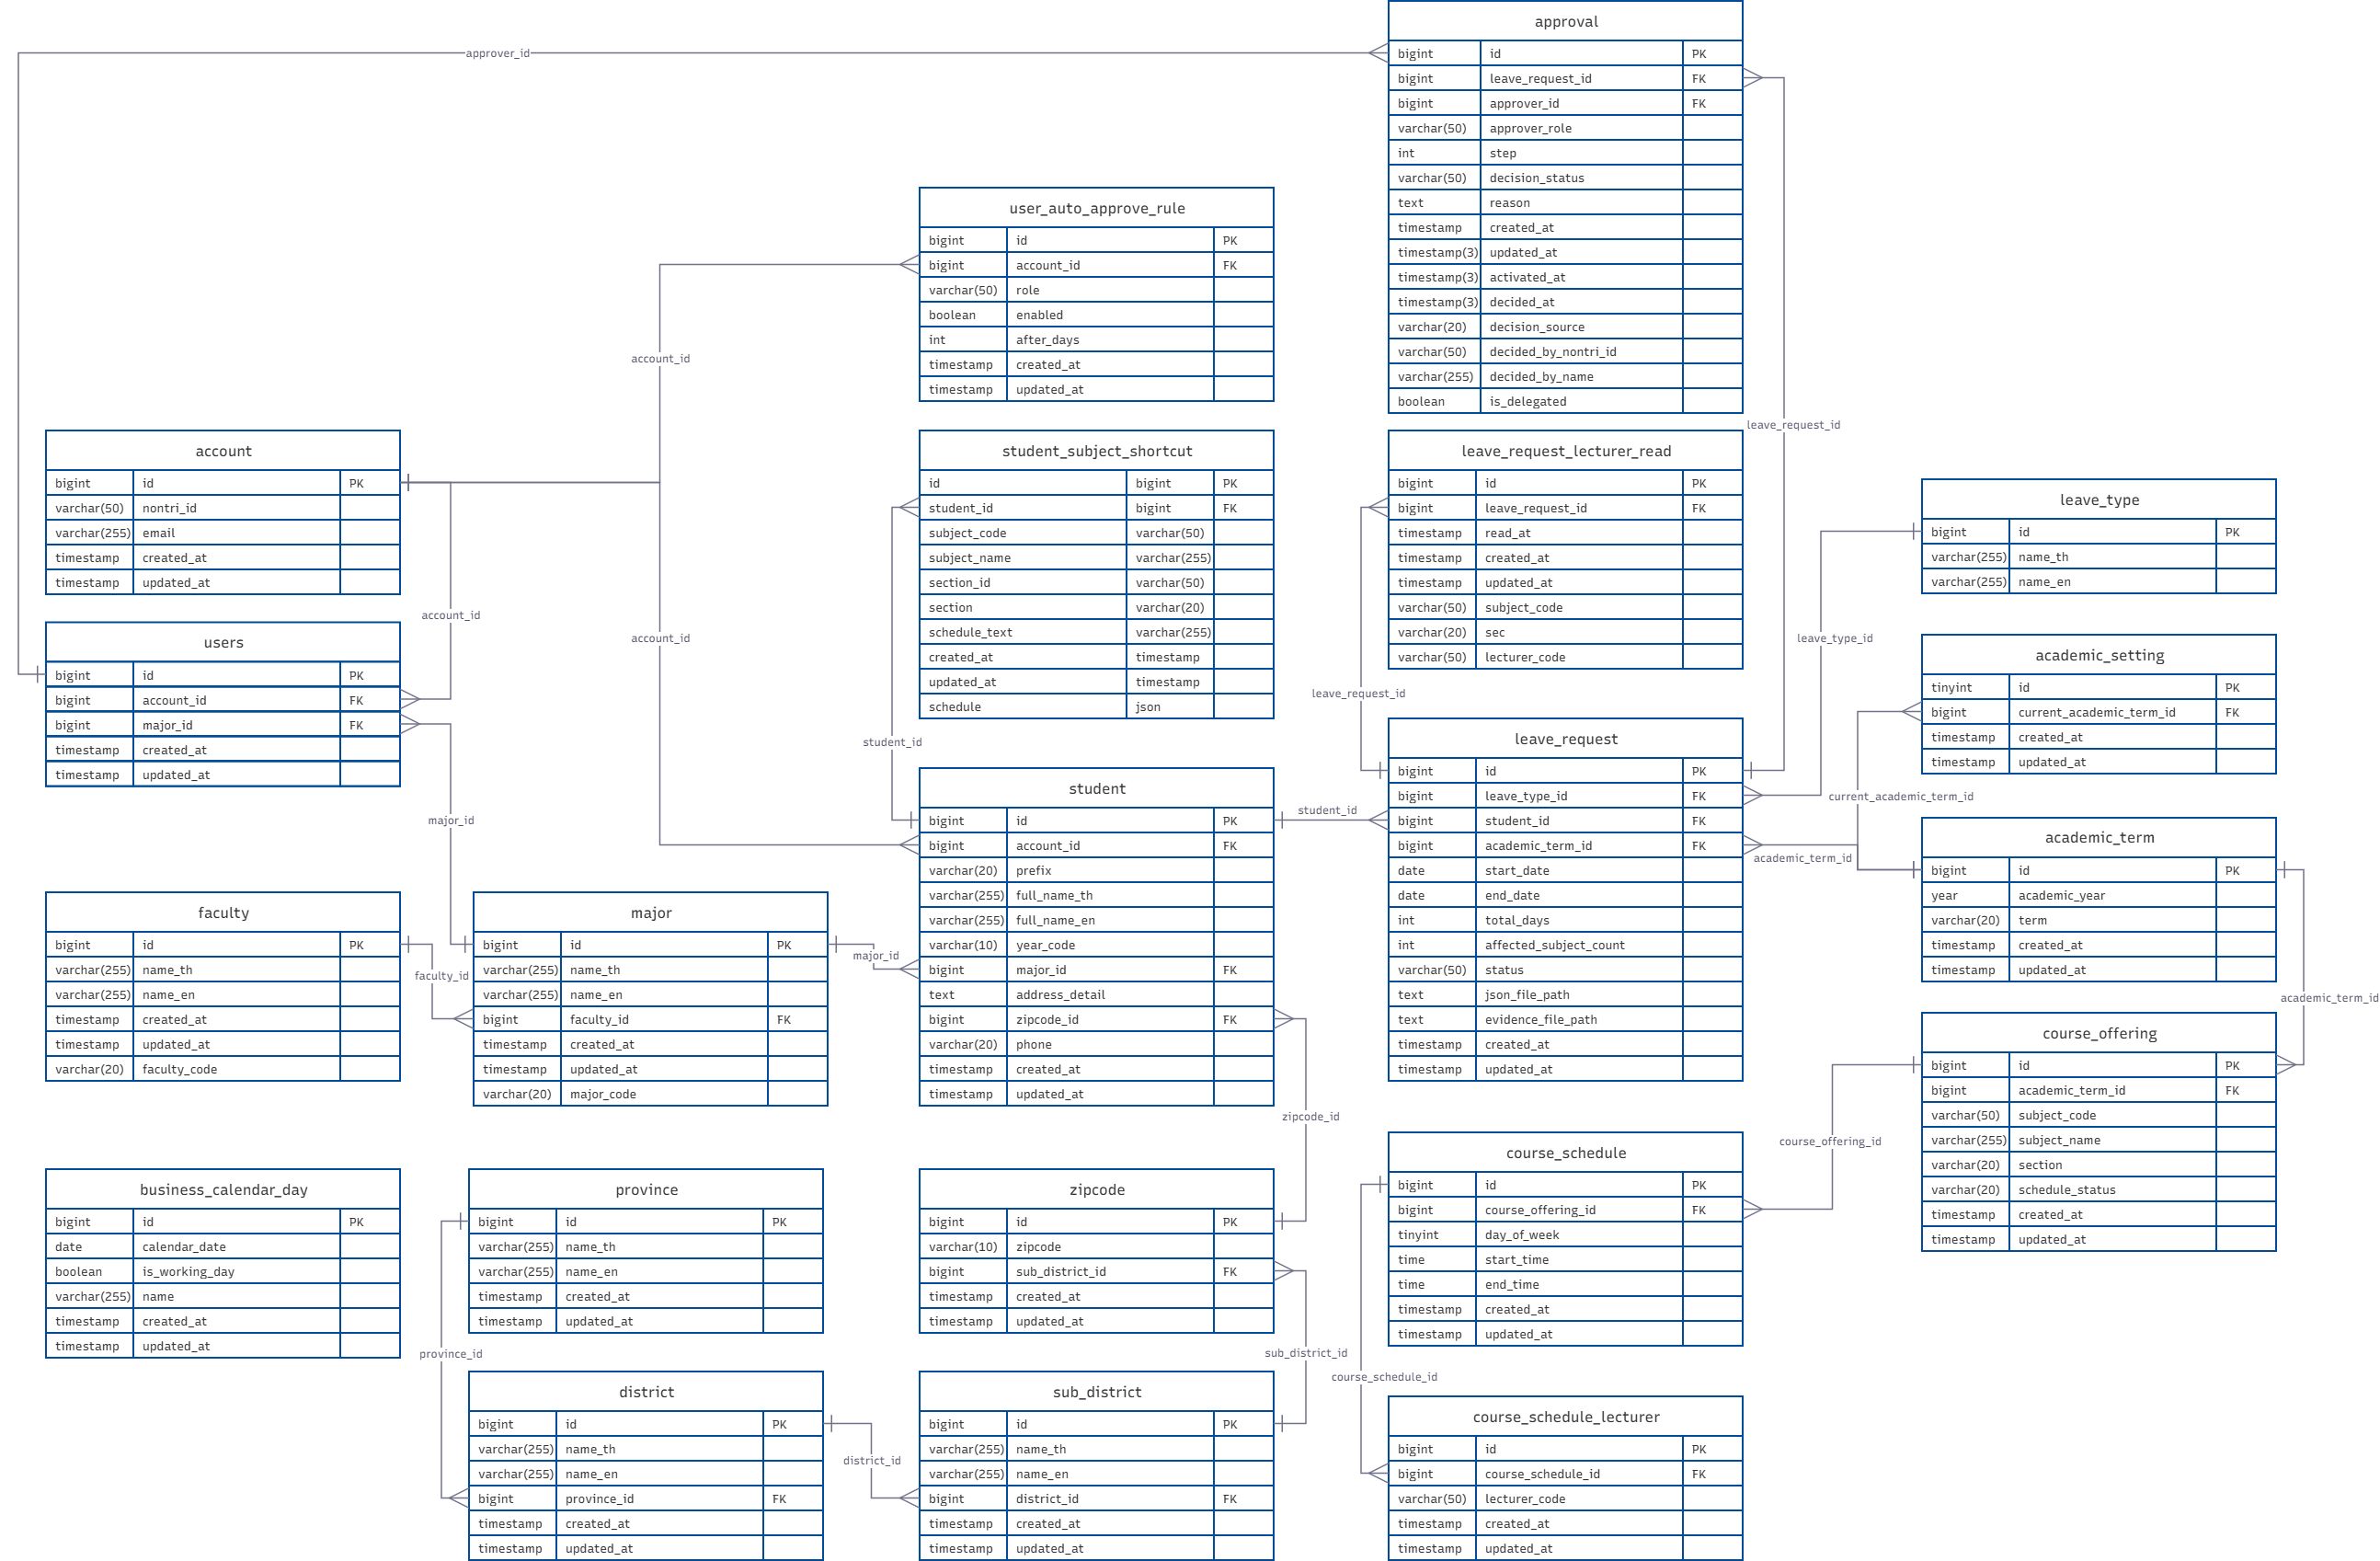
\includegraphics[width=\linewidth,height=145mm,keepaspectratio]{images/leave-schema/DB.png}
\end{center}
\clearpage
\section{ภาพรวมคลังข้อมูล (DW Overview)}
\noindent แผนภาพจากแฟ้ม \texttt{DW-OVERVIEW.png} ที่ผู้จัดทำจัดเตรียม ปรับขนาดตามสัดส่วนให้เต็มพื้นที่หน้าแนวนอน
\begin{center}
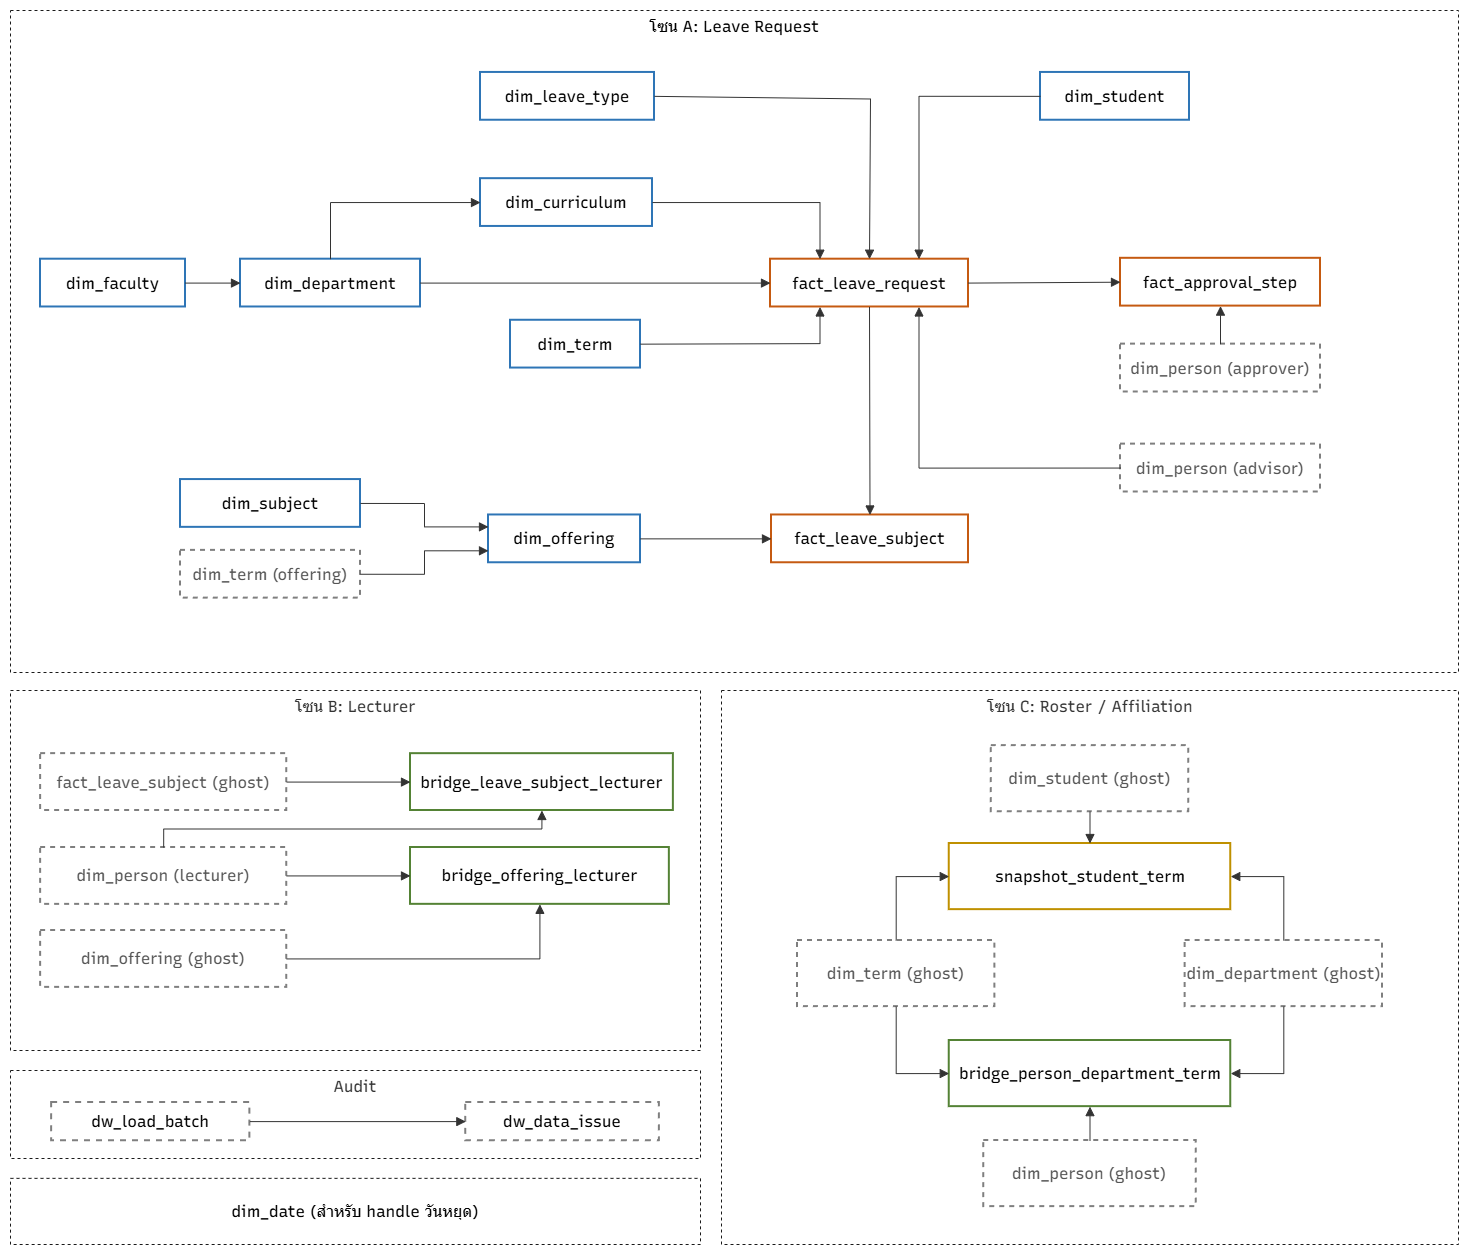
\includegraphics[width=\linewidth,height=145mm,keepaspectratio]{images/leave-schema/DW-OVERVIEW.png}
\end{center}
\clearpage
\section{แผนภาพความสัมพันธ์คลังข้อมูล (DW ERD)}
\noindent แผนภาพจากแฟ้ม \texttt{DW-ERD.png} ที่ผู้จัดทำจัดเตรียม ปรับขนาดตามสัดส่วนให้เต็มพื้นที่หน้าแนวนอน
\begin{center}
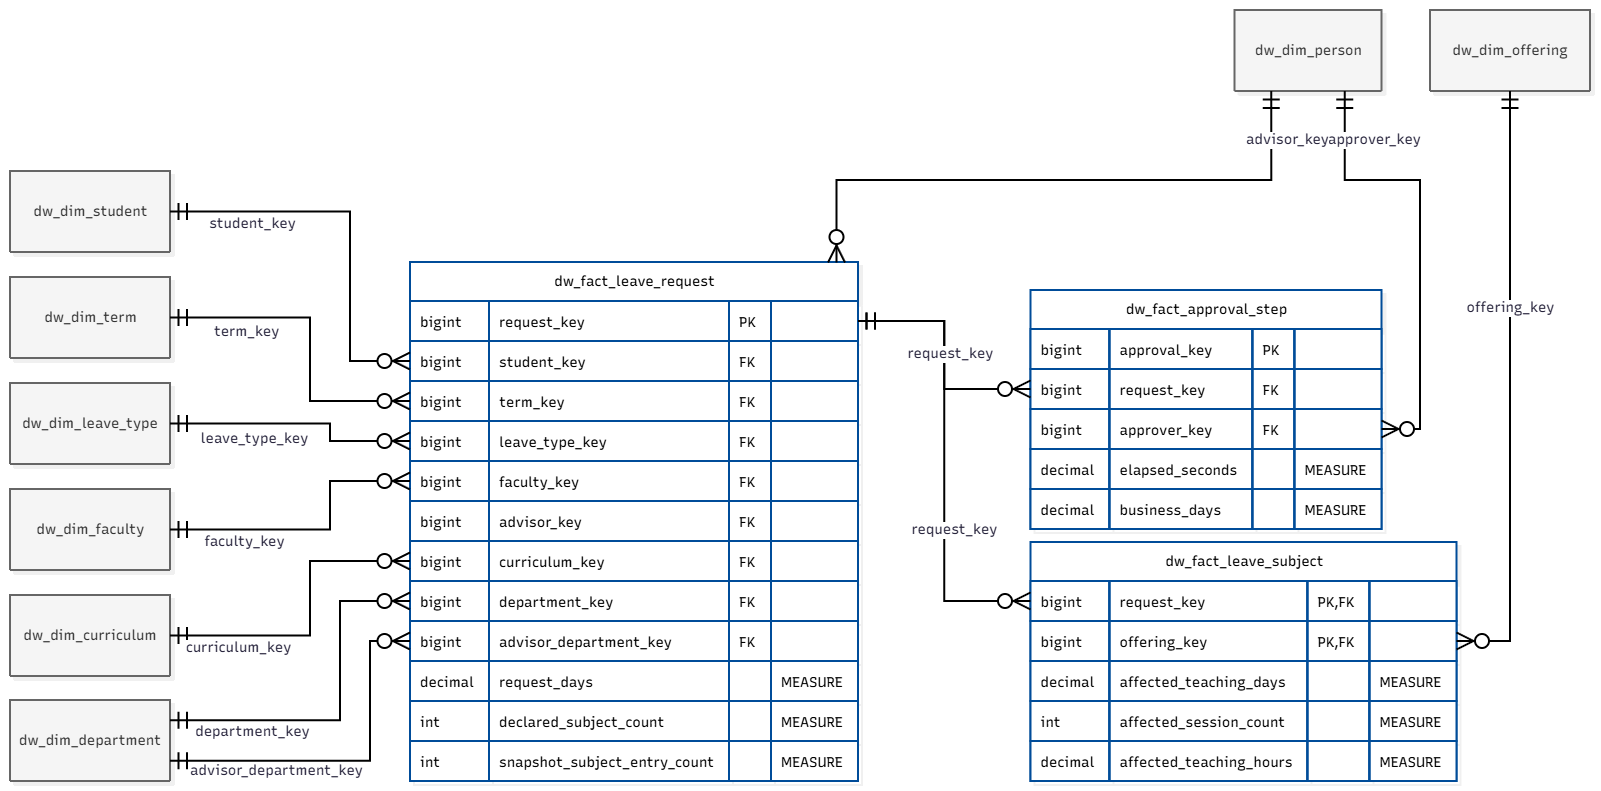
\includegraphics[width=\linewidth,height=145mm,keepaspectratio]{images/leave-schema/DW-ERD.png}
\end{center}
\clearpage
\section{แผนภาพคลังข้อมูลฉบับเต็ม รุ่นที่ 2}
\noindent แผนภาพจากแฟ้ม \texttt{DW-FULL\_VERSION\_2.png} ที่ผู้จัดทำจัดเตรียม ปรับขนาดตามสัดส่วนให้เต็มพื้นที่หน้าแนวนอน
\begin{center}
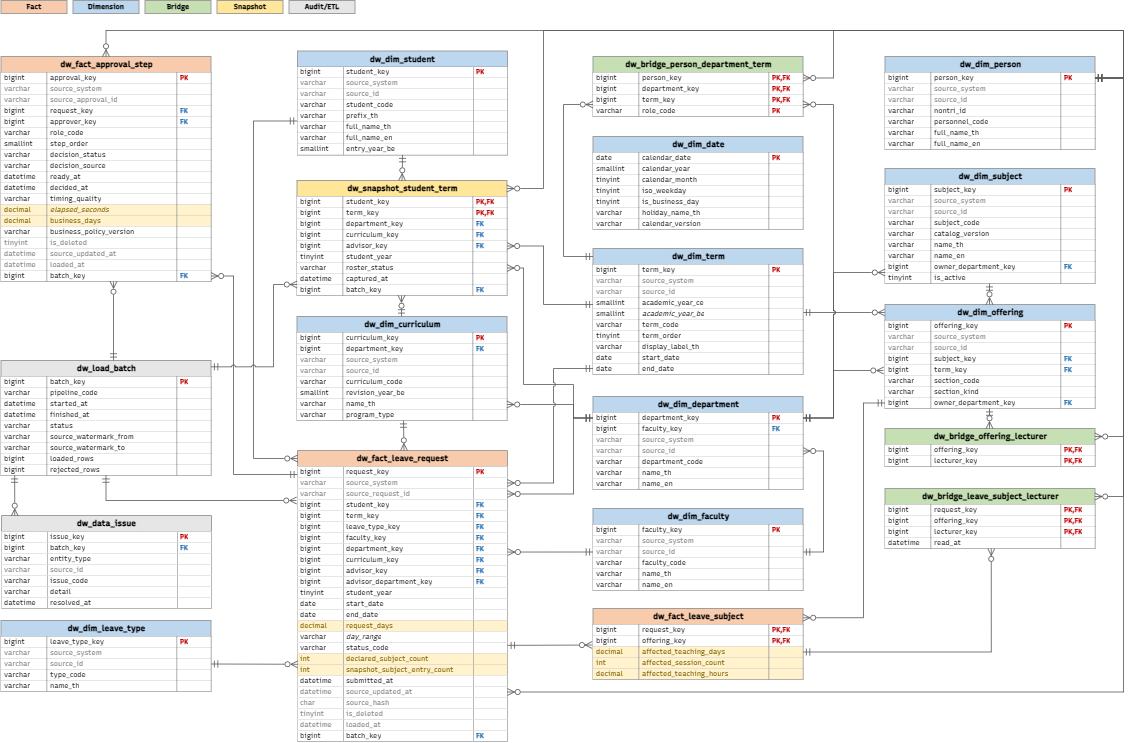
\includegraphics[width=\linewidth,height=145mm,keepaspectratio]{images/leave-schema/DW-FULL_VERSION_2.png}
\end{center}
\clearpage
\section{แผนภาพคอลัมน์ควบคุมคลังข้อมูล}
\noindent แผนภาพจากแฟ้ม \texttt{DW-CONTROL\_COLUMNS.png} ที่ผู้จัดทำจัดเตรียม ปรับขนาดตามสัดส่วนให้เต็มพื้นที่หน้าแนวนอน
\begin{center}
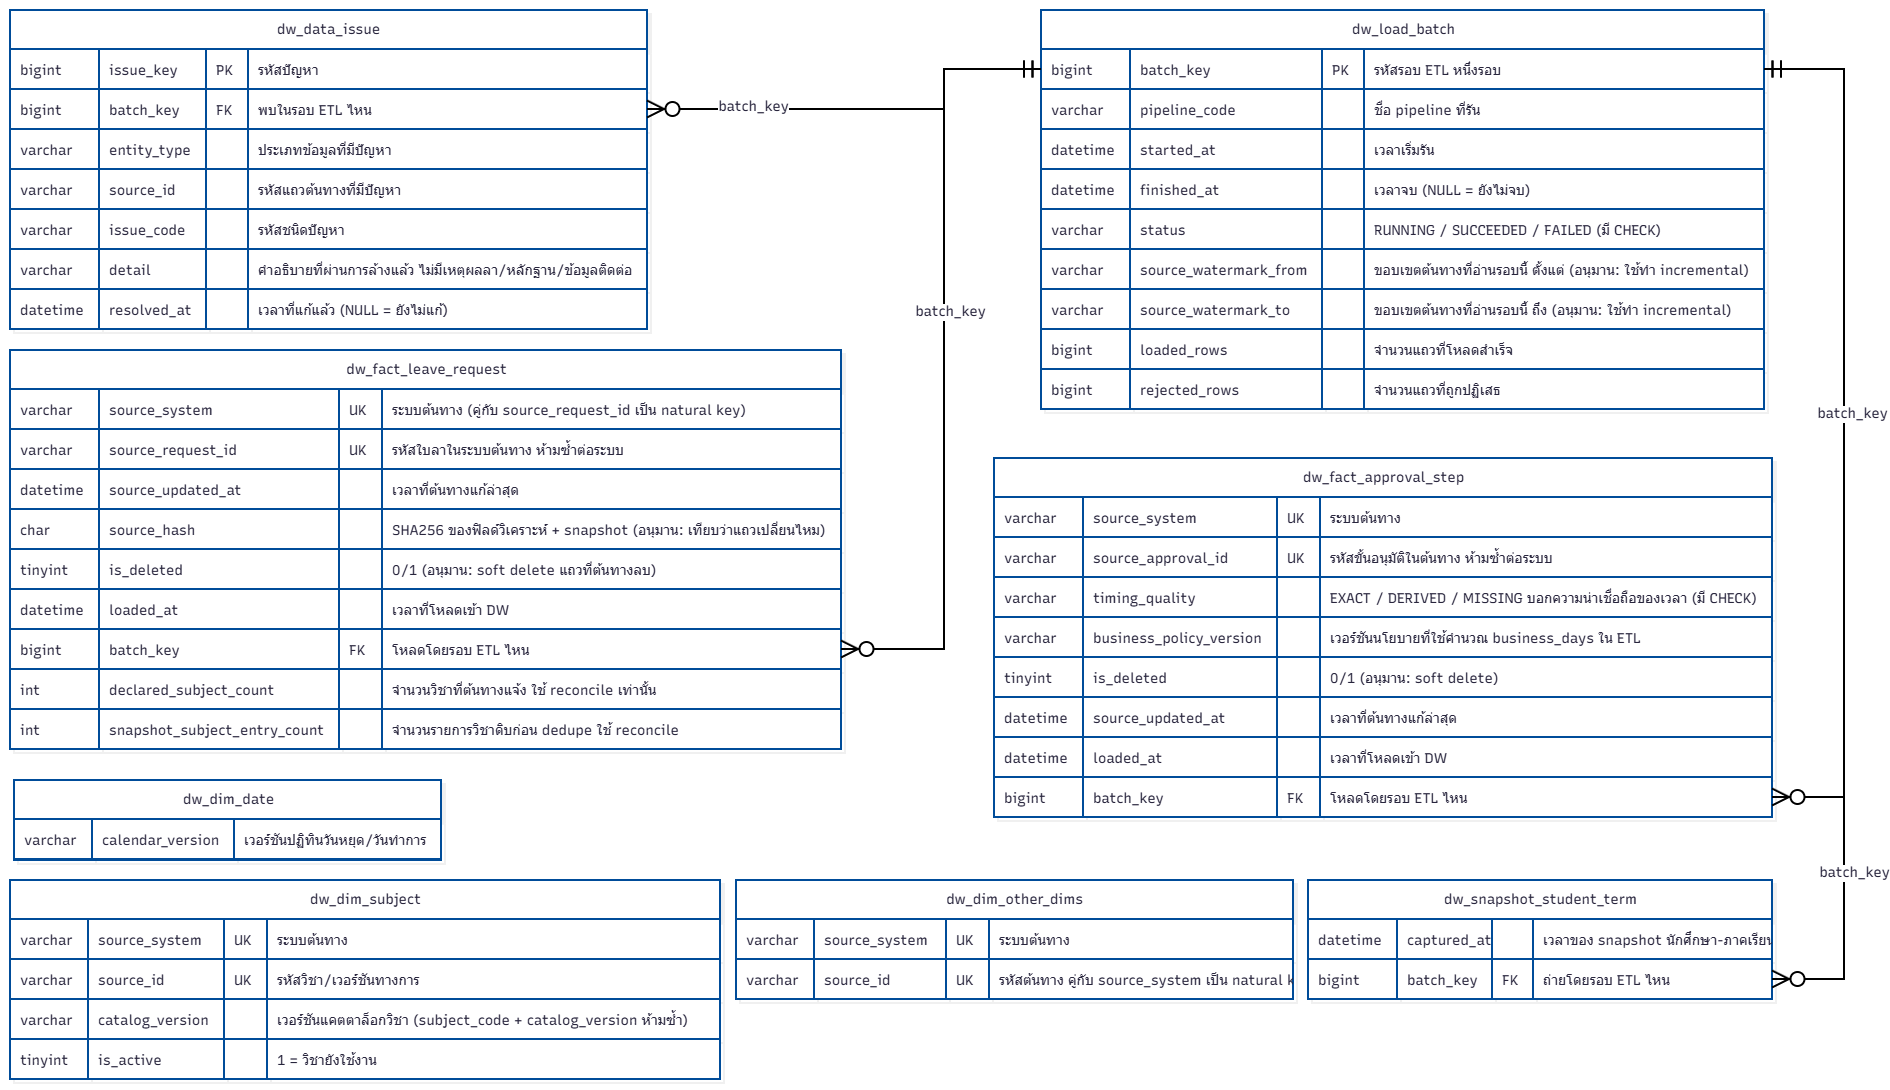
\includegraphics[width=\linewidth,height=145mm,keepaspectratio]{images/leave-schema/DW-CONTROL_COLUMNS.png}
\end{center}
\end{landscape}

\end{document}
